\documentclass[aspectratio=169,11pt]{beamer}

\usepackage[T1]{fontenc}
\usepackage[sfdefault]{FiraSans}

\usepackage{booktabs}
\usepackage{listings}
\usepackage{tikz}
\usetikzlibrary{positioning}

% --------------------------------------------------
% Colors
% --------------------------------------------------

\definecolor{WorkshopBlue}{RGB}{25,68,105}
\definecolor{WorkshopLightBlue}{RGB}{225,238,249}
\definecolor{WorkshopGreen}{RGB}{235,247,232}

% --------------------------------------------------
% Beamer appearance
% --------------------------------------------------

\setbeamertemplate{navigation symbols}{}

\setbeamercolor{normal text}{fg=black,bg=white}

\setbeamercolor{frametitle}{
    fg=white,
    bg=WorkshopBlue
}

\setbeamerfont{frametitle}{
    size=\Large,
    series=\bfseries
}

\setbeamertemplate{frametitle}{
    \nointerlineskip
    \begin{beamercolorbox}[
        wd=\paperwidth,
        ht=1.05cm,
        dp=0.25cm,
        leftskip=0.35cm
    ]{frametitle}
        \insertframetitle
    \end{beamercolorbox}
}

% --------------------------------------------------
% Footer
% --------------------------------------------------
\setbeamertemplate{footline}{
    \leavevmode
    \begin{beamercolorbox}[
        wd=\paperwidth,
        ht=0.42cm,
        dp=0.15cm
    ]{frametitle}

        \hbox to \paperwidth{

            \hspace{0.25cm}
            \scriptsize
            Chetan Adhikary \quad (Day 1)

            \hfill

            \scriptsize
            Python Workshop

            \hfill

            \scriptsize
            \insertframenumber

            \hspace{0.25cm}

        }

    \end{beamercolorbox}
}
% --------------------------------------------------
% Title information
% --------------------------------------------------

\title{Python Workshop}
\subtitle{From Python Fundamentals to a Working Application}
\author{Chetan Adhikary}
\institute{Day 1}
\date{}

\begin{document}

\input{slides/01_title}
\begin{frame}{What We Will Build}

    \begin{center}
        \Large A small \textbf{Student Management System}
    \end{center}

    \vspace{0.5cm}

    \begin{itemize}
        \item \textbf{Add} students
        \item \textbf{View \& Find} students
        \item \textbf{Update \& Delete} students
        \item \textbf{Save \& Load} student data
    \end{itemize}

    \vfill

    \begin{center}
        \textbf{Python concepts}
        \quad $\longrightarrow$ \quad
        \textbf{Application}
    \end{center}

\end{frame}
\begin{frame}{The Learning Journey}

    \begin{center}
        \Large
        \textbf{Python Concepts}
        $\longrightarrow$
        \textbf{Application Design}
        $\longrightarrow$
        \textbf{Working Application}
    \end{center}

    \vspace{0.7cm}

    \begin{itemize}
        \item \textbf{Functions} -- organize reusable logic
        \item \textbf{Modules} -- organize code into files
        \item \textbf{Exceptions} -- handle unexpected situations
        \item \textbf{Files \& JSON} -- store and retrieve data
        \item \textbf{OOP} -- model real-world entities
        \item \textbf{Application Design} -- bring everything together
    \end{itemize}

    \vfill

    \begin{center}
        \textbf{Goal:} Understand not just \emph{what} Python can do,
        but \emph{how} to use it to build an application.
    \end{center}

\end{frame}
\begin{frame}{Functions — Why Do We Need Them?}

    \begin{center}
        \Large
        \textbf{Repeated Code}
        $\longrightarrow$
        \textbf{More Changes}
        $\longrightarrow$
        \textbf{Harder to Maintain}
    \end{center}

    \vspace{0.8cm}

    \begin{itemize}
        \item Break a large problem into smaller pieces
        \item Reuse logic instead of repeating code
        \item Give a meaningful name to a piece of logic
        \item Make code easier to test and maintain
    \end{itemize}

    \vfill

    \begin{center}
        \Large
        \textbf{Problem}
        $\rightarrow$
        \textbf{Function}
        $\rightarrow$
        \textbf{Reusable Logic}
    \end{center}

\end{frame}
\begin{frame}{Modules — Why Do We Need Them?}

    \begin{center}
        \Large
        \textbf{One Large File}
        $\longrightarrow$
        \textbf{Multiple Modules}
        $\longrightarrow$
        \textbf{Organized Application}
    \end{center}

    \vspace{0.8cm}

    \begin{itemize}
        \item Split a large program into smaller files
        \item Group related functionality together
        \item Reuse code across different parts of an application
        \item Make the project easier to understand and maintain
    \end{itemize}

    \vfill

    \begin{center}
        \Large
        \textbf{Functions organize logic}
        \quad $\rightarrow$ \quad
        \textbf{Modules organize code}
    \end{center}

\end{frame}
\begin{frame}{Exceptions — When Things Go Wrong}

    \begin{center}
        \Large
        \textbf{Program}
        $\longrightarrow$
        \textbf{Unexpected Input}
        $\longrightarrow$
        \textbf{Exception}
    \end{center}

    \vspace{0.8cm}

    \begin{itemize}
        \item Programs can encounter unexpected situations
        \item User input may not be in the expected format
        \item Files may not exist
        \item External operations may fail
    \end{itemize}

    \vfill

    \begin{center}
        \Large
        \textbf{try}
        $\rightarrow$
        \textbf{Handle the problem}
        $\rightarrow$
        \textbf{Continue safely}
    \end{center}

\end{frame}
\begin{frame}{Files \& JSON — Making Data Persist}

    \begin{center}
        \Large
        \textbf{Program}
        $\longrightarrow$
        \textbf{Data in Memory}
        $\longrightarrow$
        \textbf{Program Ends}
    \end{center}

    \vspace{0.6cm}

    \begin{center}
        \Large
        \textbf{What happens to our data?}
    \end{center}

    \vspace{0.6cm}

    \begin{itemize}
        \item Files allow data to survive after the program ends
        \item JSON provides a simple format for structured data
        \item Python can write data to JSON files
        \item Python can read the data back when needed
    \end{itemize}

    \vfill

    \begin{center}
        \Large
        \textbf{Python Objects}
        $\longleftrightarrow$
        \textbf{JSON File}
    \end{center}

\end{frame}
\begin{frame}{From JSON to an Application}

    \begin{center}
        \Large
        \textbf{JSON}
        $\longrightarrow$
        \textbf{Data}
        $\longrightarrow$
        \textbf{Application Logic}
    \end{center}

    \vspace{0.8cm}

    \begin{itemize}
        \item JSON is useful for storing structured data
        \item But an application needs more than stored data
        \item We need operations such as Add, Find, Update and Delete
        \item We need a way to represent real-world entities
    \end{itemize}

    \vfill

    \begin{center}
        \Large
        \textbf{Data alone is not an application}
    \end{center}

\end{frame}
\begin{frame}{OOP — Classes \& Objects}

    \begin{columns}[T]

        % ==================================================
        % LEFT: UML DIAGRAM
        % ==================================================

        \begin{column}{0.42\textwidth}

            \vspace{0.05cm}

            \begin{center}

                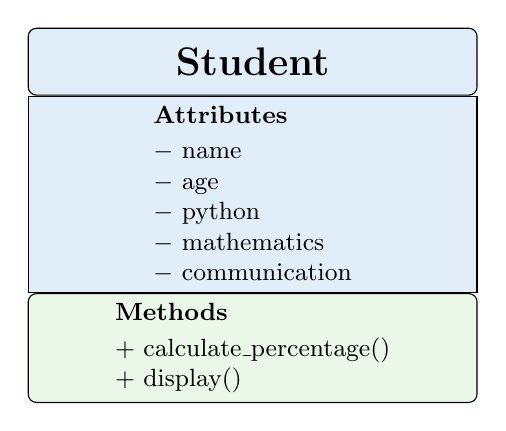
\begin{tikzpicture}[
                    font=\small
                ]

                    % -------------------------------
                    % Student header
                    % -------------------------------

                    \node[
                        draw=black,
                        fill=WorkshopLightBlue,
                        minimum width=5.7cm,
                        minimum height=0.85cm,
                        rounded corners=3pt,
                        font=\Large\bfseries
                    ] (student) {
                        Student
                    };


                    % -------------------------------
                    % Attributes
                    % -------------------------------

                    \node[
                        draw=black,
                        fill=WorkshopLightBlue,
                        minimum width=5.7cm,
                        align=left,
                        inner xsep=0.28cm,
                        inner ysep=0.12cm,
                        below=0pt of student
                    ] (attributes) {
                        \textbf{Attributes}\\[2pt]
                        $-$ name\\
                        $-$ age\\
                        $-$ python\\
                        $-$ mathematics\\
                        $-$ communication
                    };


                    % -------------------------------
                    % Methods
                    % -------------------------------

                    \node[
                        draw=black,
                        fill=WorkshopGreen,
                        minimum width=5.7cm,
                        align=left,
                        inner xsep=0.28cm,
                        inner ysep=0.12cm,
                        below=0pt of attributes,
                        rounded corners=3pt
                    ] (methods) {
                        \textbf{Methods}\\[2pt]
                        $+$ calculate\_percentage()\\
                        $+$ display()
                    };

                \end{tikzpicture}

            \end{center}

        \end{column}


        % ==================================================
        % RIGHT: EXPLANATION
        % ==================================================

        \begin{column}{0.54\textwidth}

            \vspace{0.15cm}

            \begin{itemize}

                \item
                A \textcolor{WorkshopBlue}{\textbf{class}}
                defines the structure and behavior

                \vspace{0.22cm}

                \item
                An \textcolor{WorkshopBlue}{\textbf{object}}
                is an instance of a class

                \vspace{0.22cm}

                \item
                Objects combine data (attributes) and
                operations (methods)

                \vspace{0.22cm}

                \item
                This helps us model real-world entities
                in code

            \end{itemize}

        \end{column}

    \end{columns}


    % ==================================================
    % BOTTOM SUMMARY
    % ==================================================

    \vfill

    \begin{center}

        
\begin{tikzpicture}

            \node[
                draw=WorkshopLightBlue!80!black,
                fill=WorkshopLightBlue,
                rounded corners=5pt,
                minimum width=12.8cm,
                minimum height=0.75cm
            ] {};

            \node at (-3.0,0)
            {
                \large
                \textbf{Class}
                $\rightarrow$
                Blueprint
            };

            \node at (3.0,0)
            {
                \large
                \textbf{Object}
                $\rightarrow$
                Actual Student
            };

        \end{tikzpicture}

    \end{center}

\end{frame}
\begin{frame}{Encapsulation — Controlling Access to Data}

    \begin{columns}[T]

        % ==================================================
        % LEFT: STUDENT ATTRIBUTE
        % ==================================================

        \begin{column}{0.43\textwidth}

            \begin{center}

                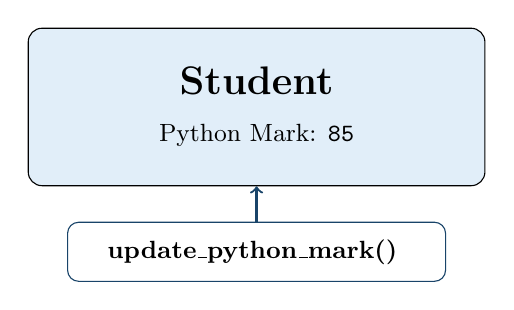
\begin{tikzpicture}[
                    font=\small
                ]

                    % Student object
                    \node[
                        draw=black,
                        fill=WorkshopLightBlue,
                        rounded corners=5pt,
                        minimum width=5.8cm,
                        minimum height=2.0cm,
                        align=center
                    ] (student) {
                        \Large\textbf{Student}\\[6pt]
                        Python Mark: \texttt{85}
                    };

                    % Controlled access
                    \node[
                        draw=WorkshopBlue,
                        fill=white,
                        rounded corners=4pt,
                        minimum width=4.8cm,
                        minimum height=0.75cm,
                        below=0.45cm of student,
                        align=center
                    ] (method) {
                        \textbf{update\_python\_mark()}
                    };

                    % Arrow
                    \draw[
                        ->,
                        thick,
                        WorkshopBlue
                    ]
                    (method.north)
                    -- (student.south);

                \end{tikzpicture}

            \end{center}

        \end{column}


        % ==================================================
        % RIGHT: EXPLANATION
        % ==================================================

        \begin{column}{0.54\textwidth}

            \vspace{0.15cm}

            \begin{itemize}

                \item Protect the object's internal data

                \vspace{0.25cm}

                \item Control how data is changed

                \vspace{0.25cm}

                \item Put validation rules in one place

                \vspace{0.25cm}

                \item Prevent invalid state where possible

            \end{itemize}

        \end{column}

    \end{columns}


    \vfill

    \begin{center}

        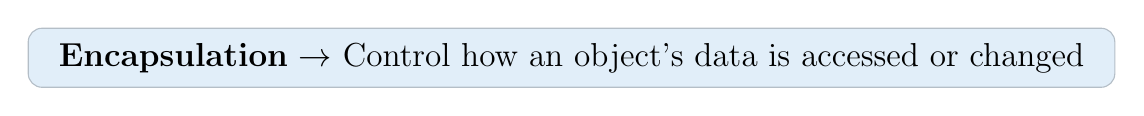
\begin{tikzpicture}

            \node[
                draw=WorkshopLightBlue!80!black,
                fill=WorkshopLightBlue,
                rounded corners=5pt,
                minimum width=13.8cm,
                minimum height=0.75cm
            ] {};

            \node {
                \large
                \textbf{Encapsulation}
                $\rightarrow$
                Control how an object's data is accessed or changed
            };

        \end{tikzpicture}

    \end{center}

\end{frame}
\begin{frame}{Inheritance — Reusing Common Behavior}

    \begin{center}

        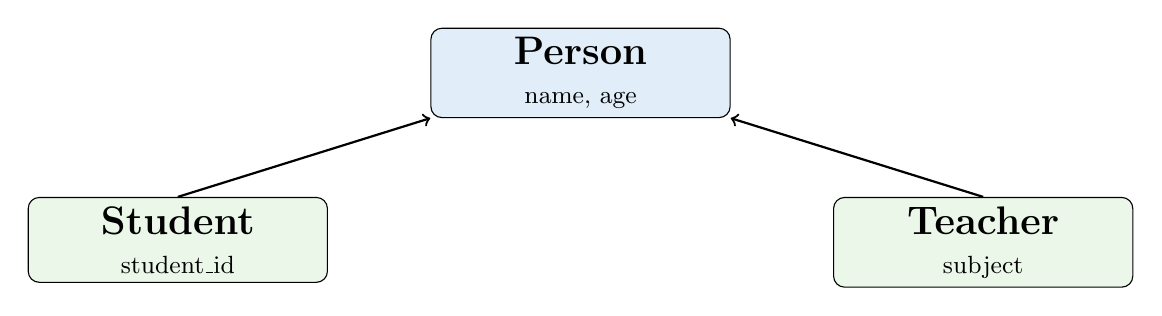
\begin{tikzpicture}[
            font=\small,
            classbox/.style={
                draw=black,
                rounded corners=4pt,
                minimum width=3.8cm,
                minimum height=1cm,
                align=center
            }
        ]

            % Parent class
            \node[
                classbox,
                fill=WorkshopLightBlue
            ] (person) {
                \Large\textbf{Person}\\[3pt]
                name,\ age
            };

            % Child classes
            \node[
                classbox,
                fill=WorkshopGreen,
                below left=1cm and 1.3cm of person
            ] (student) {
                \Large\textbf{Student}\\[3pt]
                student\_id
            };

            \node[
                classbox,
                fill=WorkshopGreen,
                below right=1cm and 1.3cm of person
            ] (teacher) {
                \Large\textbf{Teacher}\\[3pt]
                subject
            };

            % Inheritance arrows
            \draw[
                ->,
                thick
            ]
            (student.north)
            -- (person.south west);

            \draw[
                ->,
                thick
            ]
            (teacher.north)
            -- (person.south east);

        \end{tikzpicture}

    \end{center}

    \vspace{0.2cm}

    \begin{itemize}

        \item Put common attributes and behavior in a parent class

        \item Child classes inherit that common functionality

        \item Child classes can add their own attributes and behavior

    \end{itemize}

    \vfill

    \begin{center}
        \textbf{Person}
        $\rightarrow$
        \textbf{Student / Teacher}
    \end{center}

\end{frame}
\begin{frame}{From Concepts to Application Design}

    \begin{center}

        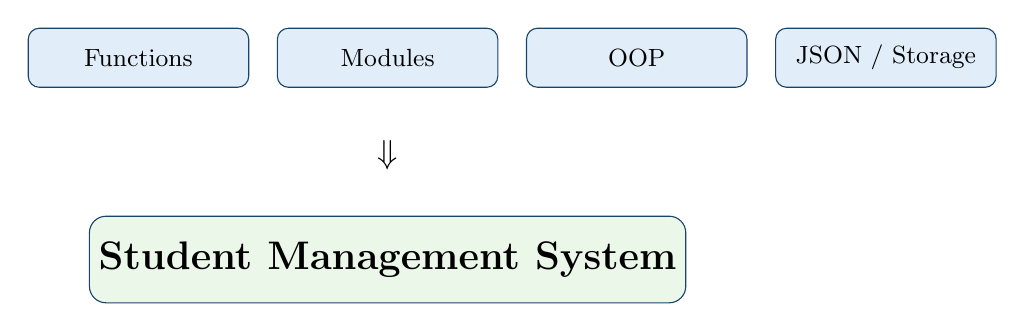
\begin{tikzpicture}[
            font=\small,
            concept/.style={
                draw=WorkshopBlue,
                fill=WorkshopLightBlue,
                rounded corners=4pt,
                minimum width=2.8cm,
                minimum height=0.75cm,
                align=center
            }
        ]

            % Concepts
            \node[concept] (functions) {Functions};
            \node[concept, right=0.35cm of functions] (modules) {Modules};
            \node[concept, right=0.35cm of modules] (oop) {OOP};
            \node[concept, right=0.35cm of oop] (storage) {JSON / Storage};

            % Arrow
            \node[
                below=0.55cm of modules,
                font=\large\bfseries
            ] (arrow) {
                $\Downarrow$
            };

            % Application
            \node[
                draw=WorkshopBlue,
                fill=WorkshopGreen,
                rounded corners=6pt,
                minimum width=7.5cm,
                minimum height=1.1cm,
                below=0.45cm of arrow,
                font=\Large\bfseries
            ] (application) {
                Student Management System
            };

        \end{tikzpicture}

    \end{center}

    \vspace{0.35cm}

    \begin{itemize}

        \item Functions organize reusable logic

        \item Modules organize the code

        \item OOP models the student and related entities

        \item JSON provides persistence

    \end{itemize}

    \vfill

    \begin{center}
        \large
        \textbf{Individual concepts become building blocks of an application.}
    \end{center}

\end{frame}
\begin{frame}{Student Management System — Architecture}

    \begin{center}

        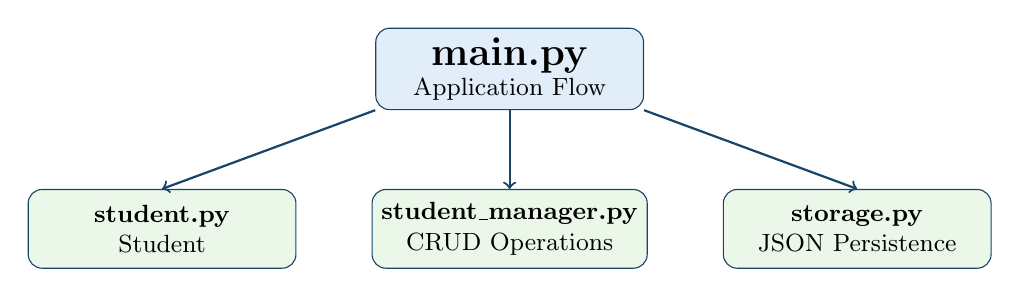
\begin{tikzpicture}[
            font=\small,
            box/.style={
                draw=WorkshopBlue,
                rounded corners=5pt,
                minimum width=3.4cm,
                minimum height=1.0cm,
                align=center
            },
            arrow/.style={
                ->,
                thick,
                WorkshopBlue
            }
        ]

            % Main application
            \node[
                box,
                fill=WorkshopLightBlue
            ] (main) {
                \Large\textbf{main.py}\\
                Application Flow
            };

            % Student
            \node[
                box,
                fill=WorkshopGreen,
                below left=1.0cm and 1.0cm of main
            ] (student) {
                \textbf{student.py}\\
                Student
            };

            % Manager
            \node[
                box,
                fill=WorkshopGreen,
                below=1.0cm of main
            ] (manager) {
                \textbf{student\_manager.py}\\
                CRUD Operations
            };

            % Storage
            \node[
                box,
                fill=WorkshopGreen,
                below right=1.0cm and 1.0cm of main
            ] (storage) {
                \textbf{storage.py}\\
                JSON Persistence
            };

            % Connections
            \draw[arrow] (main.south west) -- (student.north);
            \draw[arrow] (main.south) -- (manager.north);
            \draw[arrow] (main.south east) -- (storage.north);

        \end{tikzpicture}

    \end{center}

    \vfill

    \begin{center}
        \large
        \textbf{Each component has a clear responsibility.}
    \end{center}

\end{frame}
\begin{frame}{CRUD Operations — Managing Students}

    \begin{center}

        
\begin{tikzpicture}[
            font=\small,
            operation/.style={
                draw=WorkshopBlue,
                fill=WorkshopLightBlue,
                rounded corners=5pt,
                minimum width=2.6cm,
                minimum height=1.15cm,
                align=center
            }
        ]

            \node[operation] (create) {
                \Large\textbf{Create}\\[3pt]
                Add Student
            };

            \node[
                operation,
                right=0.45cm of create
            ] (read) {
                \Large\textbf{Read}\\[3pt]
                View / Find
            };

            \node[
                operation,
                right=0.45cm of read
            ] (update) {
                \Large\textbf{Update}\\[3pt]
                Modify Student
            };

            \node[
                operation,
                right=0.45cm of update
            ] (delete) {
                \Large\textbf{Delete}\\[3pt]
                Remove Student
            };

        \end{tikzpicture}

    \end{center}

    \vspace{0.8cm}

    \begin{center}
        \Large
        \textbf{CRUD}
        $\rightarrow$
        The basic operations needed to manage application data
    \end{center}

    \vfill

    \begin{center}
        \textbf{StudentManager} provides these operations for our application.
    \end{center}

\end{frame}
\begin{frame}{Building the Application}

    \begin{center}

        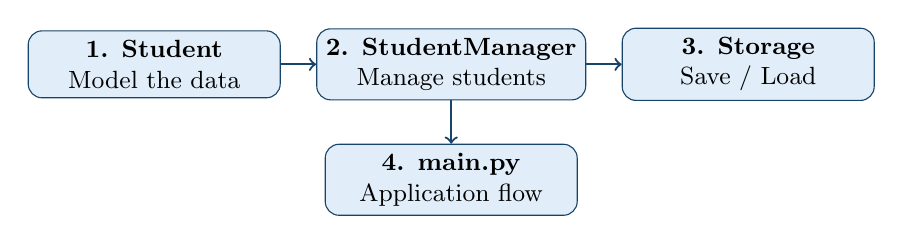
\begin{tikzpicture}[
            font=\small,
            stepbox/.style={
                draw=WorkshopBlue,
                fill=WorkshopLightBlue,
                rounded corners=5pt,
                minimum width=3.2cm,
                minimum height=0.85cm,
                align=center
            }
        ]

            \node[stepbox] (model) {
                \textbf{1. Student}\\
                Model the data
            };

            \node[
                stepbox,
                right=0.45cm of model
            ] (manager) {
                \textbf{2. StudentManager}\\
                Manage students
            };

            \node[
                stepbox,
                right=0.45cm of manager
            ] (storage) {
                \textbf{3. Storage}\\
                Save / Load
            };

            \node[
                stepbox,
                below=0.55cm of manager
            ] (main) {
                \textbf{4. main.py}\\
                Application flow
            };

            \draw[
                ->,
                thick,
                WorkshopBlue
            ]
            (model) -- (manager);

            \draw[
                ->,
                thick,
                WorkshopBlue
            ]
            (manager) -- (storage);

            \draw[
                ->,
                thick,
                WorkshopBlue
            ]
            (manager) -- (main);

        \end{tikzpicture}

    \end{center}

    \vfill

    \begin{center}
        \large
        \textbf{Build one component at a time, then connect them.}
    \end{center}

\end{frame}
\begin{frame}{Final Demonstration}

    \begin{center}

        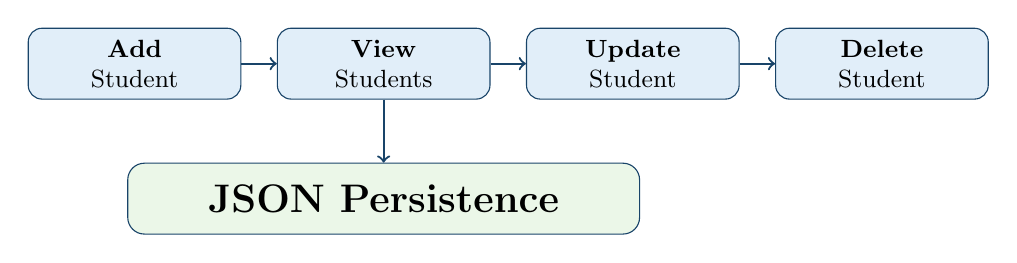
\begin{tikzpicture}[
            font=\small,
            demo/.style={
                draw=WorkshopBlue,
                fill=WorkshopLightBlue,
                rounded corners=5pt,
                minimum width=2.7cm,
                minimum height=0.9cm,
                align=center
            }
        ]

            \node[demo] (add) {
                \textbf{Add}\\
                Student
            };

            \node[
                demo,
                right=0.45cm of add
            ] (view) {
                \textbf{View}\\
                Students
            };

            \node[
                demo,
                right=0.45cm of view
            ] (update) {
                \textbf{Update}\\
                Student
            };

            \node[
                demo,
                right=0.45cm of update
            ] (delete) {
                \textbf{Delete}\\
                Student
            };

            \node[
                draw=WorkshopBlue,
                fill=WorkshopGreen,
                rounded corners=6pt,
                minimum width=6.5cm,
                minimum height=0.9cm,
                below=0.8cm of view,
                font=\Large\bfseries
            ] (persist) {
                JSON Persistence
            };

            \draw[->, thick, WorkshopBlue]
                (add) -- (view);

            \draw[->, thick, WorkshopBlue]
                (view) -- (update);

            \draw[->, thick, WorkshopBlue]
                (update) -- (delete);

            \draw[->, thick, WorkshopBlue]
                (view.south) -- (persist.north);

        \end{tikzpicture}

    \end{center}

    \vfill

    \begin{center}
        \Large
        \textbf{From Python concepts to a working application}
    \end{center}

\end{frame}
\begin{frame}{Day 1 — What We Learned}

    \begin{center}

        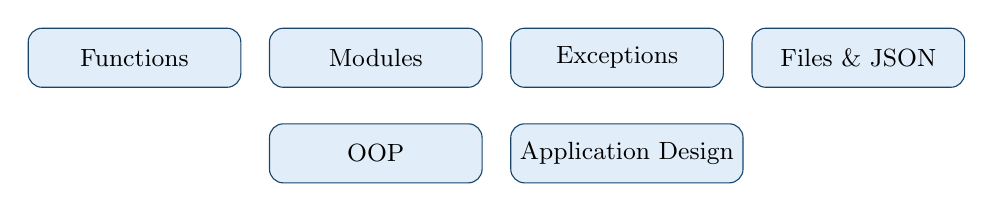
\begin{tikzpicture}[
            font=\small,
            concept/.style={
                draw=WorkshopBlue,
                fill=WorkshopLightBlue,
                rounded corners=5pt,
                minimum width=2.7cm,
                minimum height=0.75cm,
                align=center
            }
        ]

            \node[concept] (functions) {Functions};
            \node[
                concept,
                right=0.35cm of functions
            ] (modules) {Modules};
            \node[
                concept,
                right=0.35cm of modules
            ] (exceptions) {Exceptions};
            \node[
                concept,
                right=0.35cm of exceptions
            ] (files) {Files \& JSON};

            \node[
                concept,
                below=0.45cm of modules
            ] (oop) {OOP};

            \node[
                concept,
                right=0.35cm of oop
            ] (design) {Application Design};

        \end{tikzpicture}

    \end{center}

    \vspace{0.5cm}

    \begin{itemize}

        \item We moved from individual Python concepts to an application

        \item We used OOP to model real-world entities

        \item We separated responsibilities using modules

        \item We implemented CRUD operations and JSON persistence

    \end{itemize}

    \vfill

    \begin{center}
        \Large
        \textbf{Python concepts}
        $\longrightarrow$
        \textbf{Working Application}
    \end{center}

\end{frame}

\end{document}